\documentclass{article}
 \usepackage{ocgx}
 \usepackage{bookmark}
 \usepackage{amsmath}
 \usepackage{amsthm}
 \usepackage{amssymb}
 \usepackage{tikz}
 \usepackage{tikz-cd}
 \usepackage{pgfplots}
 \usepackage[utf8]{inputenc}
 \usepackage{amsfonts}
 \usepackage[margin=2.5cm]{geometry}
 \usepackage{graphicx}
 \usepackage[export]{adjustbox}
 \usepackage{fancyhdr}
 \usepackage{babel}
 \usepackage{hyperref}
 \usepackage{multirow}
 \usepackage{lastpage}
 \usepackage{mathtools}
 \usepackage{geometry}
 \usepackage{sansmathfonts}
 \usepackage{subfiles}
 \usepackage[T1]{fontenc}
\usetikzlibrary{positioning, calc, shapes.geometric, shapes.multipart, shapes, arrows.meta, arrows, decorations.markings, external, trees}
 \tikzstyle{Arrow} = [
%Create custom arrow style:
thick,
decoration={
markings,
mark=at position 1 with {
\arrow[thick]{latex}
}
},
shorten >= 3pt, preaction = {decorate}
]
 \fancyhf{}

 \pgfplotsset{compat = 1.18}

 \hypersetup{
     colorlinks,
     citecolor=black,
     filecolor=black,
     linkcolor=black,
     urlcolor=black
 }
 \newtheorem*{def*}{\underline{Definition}}
 \newtheorem*{theorem*}{\underline{Theorem}}
 \newtheorem*{lemma*}{\underline{Lemma}}
 \newtheorem*{prop*}{\underline{Proposition}}
 \newtheorem{example}{\underline{Example}}
 \newtheorem*{proof*}{\underline{Proof}}
 \newtheorem*{crl*}{\underline{Corollary}}
 \renewcommand\qedsymbol{$\blacksquare$}

 \geometry{a4paper, left=3cm, top=3cm, right=3cm, bottom=3cm}

 \rfoot{Página \thepage \hspace{1pt} de \pageref{LastPage}}

\begin{document}
\begin{figure}[ht]
	\minipage{0.76\textwidth}
	
\includegraphics[width=4cm]{../icmc.png}
	\hspace{7cm}
	
\includegraphics[height=4.9cm,width=4cm]{../brasao_usp_cor.jpg}
	\endminipage
\end{figure}

\begin{center}
	\vspace{1cm}
	\LARGE
	UNIVERSIDADE DE SÃO PAULO

	\vspace{1.3cm}
	\LARGE
	INSTITUTO DE CIÊNCIAS MATEMÁTICAS E COMPUTACIONAIS - ICMC

	\vspace{1.7cm}
	\Large
	\textbf{Subobject Classifiers, Sheaves and Topoi}

	\vspace{1.3cm}
	\large
	\textbf{Renan Wenzel - 11169472}

	\vspace{1.3cm}
	\large
	\textbf{Professor(a): Behrooz Mirzaii}

	\textbf{E-mail: bmirzaii@gmail.com}

	\vspace{5.3cm}
	\today
\end{center}

\newpage
\tableofcontents

\newpage
\section{Why Topoi? And how did they come to be?}
During the 20th century, after disccusions of the likes of Zermelo-Franklin axiomatization, the Axiom of Choice, and all things Set-Theoretical, one of the guys responsible for developing Category Theory, Bill Lawvere, wanted to really put in the \textit{foundational} part in Category Theory as a foundational theory of mathematics. For that matter, he looked at what comes to mind for most people when they think of the foundations of mathematics - sets; or, more specifically, the category Sets.

Throughout a usual mathematics formation, a student (hopefully) comes across many different areas where mathematics is done: topology, ring theory, group theory, geometry, linear algebra, analysis, and so on, and even though they are so different as to polarize those who undertake the task of understanding each are, there is a commong element behind all of them - sets, and so they are usually seen as ``something where you can do math'': add a specific type of collection of subsets and you get topology, put in some operations and you go to algebra, or start working with \(\delta \)'s and \(\varepsilon \)'s and you go to Analysis. However, the usual characterization of sets make use of, well, sets themselves, and memberships (the whole discussion of the Russel paradox was exactly a set with ambiguous membership). But when one looks at category theory, there is a different kind of discussion - instead of working with memberships and sets, one works with Objects and Morphisms, which are more general than the former. As a consequence, it is only natural to think ``Is the category of Sets NEEDED to do things regarding mathematics? Are there other options?''.

To give a taste of the disccusion that is to come, let us recall briefly a few of the axioms of Set Theory (ZFC), although informally, as Leinster does in his 2011 web-article:
\begin{itemize}
	\item there are some things called 'sets';
	\item there is a binary relation `\(\in\)';
	\item some axioms hold.
\end{itemize}

The description of the category Sets, on the other hand, goes more like:
\begin{itemize}
	\item there are some objects called 'sets';
	\item there are arrows going from one set to another or to itself;
	\item these arrows can become connected to form new ones via a binary relation `\(\circ \)';
	\item some axioms hold.
\end{itemize}

Throughout a course in Category Theory, those axioms mentioned in the second description become more clear, but it still holds a difference when compared to the usual ZFC: we define sets and functions/morphisms instead of sets and membership. This by itself does not seem like much, but the fact that it is done purely with categorical language means we need not to restrain ourselves to only Sets, it gives a hint on how to generalize the nice things about set theory to other categories - the possibility of doing math in other places!

Making use of the word places mentioned last paragraph, the name of this kind of generalized sets comes from the greek word for `place' - \textit{topos}[\(\tau\text{ó}\pi \mathrm{o}\zeta \), which can also mean `line of argument', very close to the kind of discussion originating topos theory!] - coined by Grothendieck while exploring this exact question of where else can we discuss mathematics in detail. More specifically, Grothendieck was exploring algebraic geometry and, more than just finding out whether or not something is true, he wanted to discover \textit{where} it is true, and that was very appealing to Lawvere. Hence, topos theory did not arise as an attempt to generalize sets; instead, it was a nice consequence of studying algebraic geometry problems.

In the end, Lawvere and his pal Tierney coined the term elementary topos to refer to this kind of generalized set and left Grothendieck Topos to refer to the idea from algebraic geometry, and they don't need the law of excluded middle (proofs by contradiction) neither the axiom of choice, ending the idea of truth as a yes-or-no affair and keeping track of how true something is. For this reason, there is current research in other areas of knowledge that are looking at topos theory as a way of unifing seemingly separate fields of knowledge and studying it from an epistemological perspective (c.f. \cite{stern2013} for the beggining of such a discussion), and (hopefully) this will lay the foundation for the end of the false trichotomy between humanities, biological, and exact sciences!

\section{Prerequisite Notions}
Given a category \(\mathcal{C}\), an object A of \(\mathcal{C}\), and two monomorphisms leaving from other object into A, say \(f:D\rightarrow A\) and \(g:E\rightarrow A\), define the following equivalence relation:
\[
	f\equiv g \Longleftrightarrow \exists\; \varphi:D\rightarrow E: f = g \circ \varphi,
\]
where \(\varphi \) is an isomorphism.

In other words, the following diagrams are commutative in \(\mathcal{C}\)
\begin{center}
	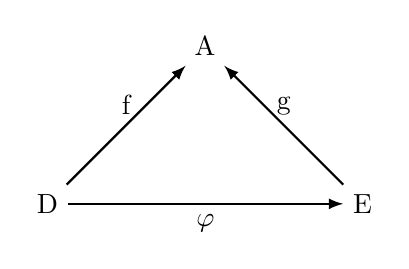
\begin{tikzpicture}[
			observed/.style = {rectangle, thick, text centered, draw, text width = 6em},
			latent/.style = {ellipse, thick, draw, text centered, text width = 6em},
			error/.style ={circle, thick, draw, text centered},
			confounding/.style = {rectangle, thick, text centered, draw, text width = 6em, minimum width = 5.5in},
			outcome/.style = {rectangle, thick, draw, text centered, minimum height = 3.5in, text width = 6em},
		]

		\node(T) at (0,1){A};
		\node(BL) at (-2,-1){D};
		\node(BR) at (2,-1){E};

		\draw[Arrow](BL)--node[midway, above] {f}(T);
		\draw[Arrow](BR)--node[midway, above] {g}(T);
		\draw[Arrow](BL)--node[midway, below] {\(\varphi \)}(BR);

	\end{tikzpicture}
\end{center}
\begin{center}
	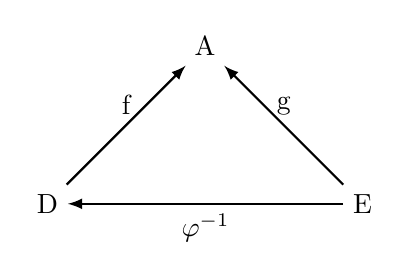
\begin{tikzpicture}[
			observed/.style = {rectangle, thick, text centered, draw, text width = 6em},
			latent/.style = {ellipse, thick, draw, text centered, text width = 6em},
			error/.style ={circle, thick, draw, text centered},
			confounding/.style = {rectangle, thick, text centered, draw, text width = 6em, minimum width = 5.5in},
			outcome/.style = {rectangle, thick, draw, text centered, minimum height = 3.5in, text width = 6em},
		]

		\node(T) at (0,1){A};
		\node(BL) at (-2,-1){D};
		\node(BR) at (2,-1){E};

		\draw[Arrow](BL)--node[midway, above] {f}(T);
		\draw[Arrow](BR)--node[midway, above] {g}(T);
		\draw[Arrow](BR)--node[midway, below] {\(\varphi^{-1} \)}(BL);
	\end{tikzpicture}
\end{center}
\begin{def*}
	Given a category \(\mathcal{C}\) and an object A in it, the \textbf{subobjects of A} are the equivalence classes of the monomorphisms from above: a subobject of A is an object \(\overline{B}\) such that
	\[
		\overline{B}=\{f, g\in \mathrm{MonHom}(D, A) \cup \mathrm{MonHom}(E, A): \exists \varphi :D\rightarrow E \text{ iso. },\; f=g\circ \varphi  \; \& \; g = f\circ \varphi^{-1}\}.
	\]
	for any objects D, E of \(\mathcal{C}\).\(\square\)
\end{def*}
In Sets, they are the subsets; in Grps, they are subgroups; and, in Top, they are subspaces.

\begin{def*}
	Let X and Y be objects of a category \(\mathcal{C}\) where all binary products with Y exist. Then, an \textbf{exponential object} is an object \(X^{Y}\) equipped with a morphism known as the \textbf{evaluation map} \(ev:X^{Y}\times Y\rightarrow X\) satisfying the following universal property: for every object Z and every map \(e:Z\times Y\rightarrow X\), there exists a unique map \(u:Z\rightarrow X^{Y}\) such that
	\[
		ev\circ (u\times \mathrm{id}_{Y}) = e,
	\]
	\textit{i.e.} the following diagram commutes:
	\begin{center}
		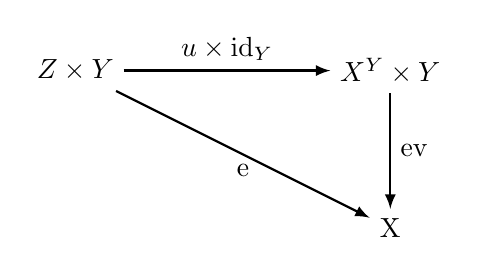
\begin{tikzpicture}[
				observed/.style = {rectangle, thick, text centered, draw, text width = 6em},
				latent/.style = {ellipse, thick, draw, text centered, text width = 6em},
				error/.style ={circle, thick, draw, text centered},
				confounding/.style = {rectangle, thick, text centered, draw, text width = 6em, minimum width = 5.5in},
				outcome/.style = {rectangle, thick, draw, text centered, minimum height = 3.5in, text width = 6em},
			]

			\node(T) at (2,1){\(X^{Y}\times Y\)};
			\node(BL) at (-2,1){\(Z\times Y\)};
			\node(BR) at (2,-1){X};

			\draw[Arrow](BL)--node[midway, above] {\(u\times \mathrm{id}_{Y}\)}(T);
			\draw[Arrow](T)--node[midway, right] {ev}(BR);
			\draw[Arrow](BL)--node[midway, below] {e}(BR);

		\end{tikzpicture}
	\end{center}
\end{def*}
this definition essentially creates a natural isomorphism between \(\mathrm{Hom}_{\mathcal{C}}(-, X^{Y})\) the set of morphisms from any object into \(X^{Y}\) and the set of morphisms from the product between any object and Y into X \(\mathrm{Hom}_{\mathcal{C}}(-\times Y, X)\), with ev being the image of the identity arrow on \(X^{Y}\).

\begin{example}
	\begin{itemize}
		\item[1)] In the case of Sets, the category, if we study the object \(X^{Y}\) with its evaluation \(ev:X^{Y}\times Y\rightarrow X\) for sets X and Y, we need another set A and a map \(e:A\times Y\rightarrow X\). Then, the equality becomes
		      \[
			      ev((u, 1))(z, y) = e(x, y).
		      \]
		      Hence, evaluation of an element in \(X^{Y}\times Y\) gives a function \(e(x, y)\) from any set into X. In other words, the exponentiation object \(X^{Y}\) in Sets is the set of functions from X to Y.
		\item[2)] There is a very nice way of giving an interpretation to the fact that \(a^{0}=1\) for any natural number a using exponentiation of categories. To do that, we consider the category of finite sets, FinSets, and the cardinality operation which takes a finite set and yields its size \(|-|:\mathrm{FinSets}\rightarrow \mathbb{N}\). The exponentiation here is given by
		      \[
			      \bigl\vert X^{S} \bigr\vert = |X|^{|S|},
		      \]
		      so that exponentiating numbers is related to the exponentiation in categories. If we denote by a fancy number the ammount of elements in a finite set, for instance \(\mathfrak{3} = |\{0, 1, 2\}|\), then the exponentiation of two finite sets \(\mathfrak{a}\) and \(\mathfrak{b}\) is given by
		      \[
			      |\mathfrak{a}^{\mathfrak{b}}| = |\mathfrak{a}|^{|\mathfrak{b}|} = a^{b}.
		      \]
		      Since the empty set is a finite set, it is an object in FinSets; in fact, an initial object at that: it has a single morphism from itself to any other finite set, and \(\emptyset = \mathfrak{0}\) because it has 0 elements. Thus,
		      \[
			      a^{0} = |\mathfrak{a}^{|\emptyset |}| = \#\text{arrows from }\emptyset\text{ to }\mathfrak{a} = 1.
		      \]
	\end{itemize}
\end{example}

\begin{def*}
	A \textbf{cartesian closed category} \(\mathcal{C}\) is one that satisfies the following properties:
	\begin{itemize}
		\item[1)] It has a \textit{terminal object};
		\item[2)] Any two objects X, Y of \(\mathcal{C}\) have a product \(X\times Y\) that is also in \(\mathcal{C}\);
		\item[3)] Any two objects Y, Z of \(\mathcal{C}\) have an \textit{exponential} \(Z^{Y}\) in \(\mathcal{C}\). \(\square\)
	\end{itemize}
\end{def*}

\begin{def*}
	A \textbf{pullback} is the limit of a diagram of two morphisms with a common codomain, i.e.,
	\begin{center}
		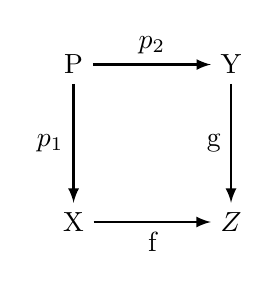
\begin{tikzpicture}[
				observed/.style = {rectangle, thick, text centered, draw, text width = 6em},
				latent/.style = {ellipse, thick, draw, text centered, text width = 6em},
				error/.style ={circle, thick, draw, text centered},
				confounding/.style = {rectangle, thick, text centered, draw, text width = 6em, minimum width = 5.5in},
				outcome/.style = {rectangle, thick, draw, text centered, minimum height = 3.5in, text width = 6em},
			]
			\node(S1) at (-2,0){P};
			\node(S2) at (-2,-2){X};
			\node(IS) at (0,0){Y};
			\node(PD) at (0,-2){\(Z\)};

			\draw[Arrow](S1)--node[midway, left] {\(p_1\)}(S2);
			\draw[Arrow](S1)--node[midway, above] {\(p_2\)}(IS);
			\draw[Arrow](IS)--node[midway, left] {g}(PD);
			\draw[Arrow](S2)--node[midway, below] {f}(PD);
		\end{tikzpicture}
	\end{center}
	where the diagram is commutative, called the \textbf{pullback square}, and the pullback \((P, p_{1}, p_{2})\) is unique up to isomorphism. \(\square\)
\end{def*}
The object P might also be called the \textbf{pullback}, depending on the context and on the authors choice, and the idea behind a pullback is the ability of creating an object with maps from two already known objects, and from that, be able to work back to the previous relationship. To bring it dows a level, in the context of Sets, if we take functions \(f:A\rightarrow C\) and \(g:B\rightarrow C\), then the pullback of this diagram is the subset \(X\subseteq A\times B\) together with arrows \((a, b)\overbracket[0pt]{\rightarrow}^{p_{1}}a\in A\) and \((a, b)\overbracket[0pt]{\rightarrow}^{p_{2}}b\in B\) such that
\[
	f(a)=g(b)
\]
holds true, i.e., X is the set of elements from \(A\times B\) to which the above holds, and \((X, p_{1}, p_{2})\) is the pullback of the diagram
\begin{center}
	\begin{tikzpicture}[
			observed/.style = {rectangle, thick, text centered, draw, text width = 6em},
			latent/.style = {ellipse, thick, draw, text centered, text width = 6em},
			error/.style ={circle, thick, draw, text centered},
			confounding/.style = {rectangle, thick, text centered, draw, text width = 6em, minimum width = 5.5in},
			outcome/.style = {rectangle, thick, draw, text centered, minimum height = 3.5in, text width = 6em},
		]

		\node(T) at (0,-1){C};
		\node(BL) at (-2,1){A};
		\node(BR) at (2,1){B};

		\draw[Arrow](BL)--node[midway, above] {f}(T);
		\draw[Arrow](BR)--node[midway, above] {g}(T);

	\end{tikzpicture}
\end{center}
which then becomes
\begin{center}
	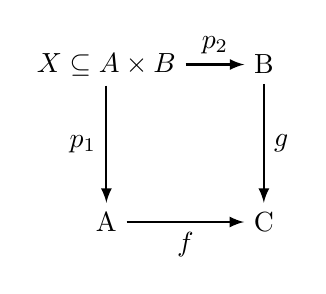
\begin{tikzpicture}[
			observed/.style = {rectangle, thick, text centered, draw, text width = 6em},
			latent/.style = {ellipse, thick, draw, text centered, text width = 6em},
			error/.style ={circle, thick, draw, text centered},
			confounding/.style = {rectangle, thick, text centered, draw, text width = 6em, minimum width = 5.5in},
			outcome/.style = {rectangle, thick, draw, text centered, minimum height = 3.5in, text width = 6em},
		]
		\node(TL) at (-1,1){\(X\subseteq A\times B\)};
		\node(BL) at (-1,-1){A};
		\node(TR) at (1,1){B};
		\node(BR) at (1,-1){C};

		\draw[Arrow](TL)--node[midway, above] {\(p_{2}\)}(TR);
		\draw[Arrow](BL)--node[midway, below] {\(f\)}(BR);
		\draw[Arrow](TL)--node[midway, left] {\(p_{1}\)}(BL);
		\draw[Arrow](TR)--node[midway, right] {\(g\)}(BR);
	\end{tikzpicture}
\end{center}
\begin{def*}
	Let \(\varepsilon \) be a category with finite limits. A \textbf{subobject classifier/truth value object} in \(\varepsilon \) is an object \(\Omega \) together with a map \(t:T\rightarrow \Omega \) such that for every monomorphism \(m:A \rightarrowtail X\) (also stated as ``for every part \(A\overbracket[0pt]{\hookrightarrow}^{m}X\) of X''), there exists a unique map \(\chi :X\rightarrow \Omega \) such that
	\begin{center}
		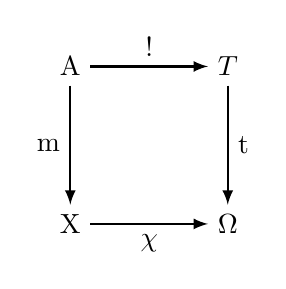
\begin{tikzpicture}[
				observed/.style = {rectangle, thick, text centered, draw, text width = 6em},
				latent/.style = {ellipse, thick, draw, text centered, text width = 6em},
				error/.style ={circle, thick, draw, text centered},
				confounding/.style = {rectangle, thick, text centered, draw, text width = 6em, minimum width = 5.5in},
				outcome/.style = {rectangle, thick, draw, text centered, minimum height = 3.5in, text width = 6em},
			]
			\node(TL) at (-1,1){A};
			\node(BL) at (-1,-1){X};
			\node(TR) at (1,1){\(T\)};
			\node(BR) at (1,-1){\(\Omega \)};

			\draw[Arrow](TL)--node[midway, above] {!}(TR);
			\draw[Arrow](BL)--node[midway, below] {\(\chi \)}(BR);
			\draw[Arrow](TL)--node[midway, left] {m}(BL);
			\draw[Arrow](TR)--node[midway, right] {t}(BR);

		\end{tikzpicture}
	\end{center}
	is a \textit{pullback square}; it should be noted that ! means the terminal map to the terminal object T - the single element in \(\mathrm{Hom}(A, T)\) - and t is usually called ``true''. \(\square\)
\end{def*}

\begin{example}
	\begin{itemize}
		\item[1)] In the context of Sets, where the terminal object is a singleton set, looking for the subobject classifier would be the same as looking for a unique function such that x is included in a part of a set if and only if that function ``holds true'': if X is a set and \(A\subseteq X\) is a part of X (there is an inclusion/injective function from A to X), we´d look for the only function \(t:A\rightarrow \{\text{true}, \text{false}\}\) such that for all elements a of A, the function would answer the question ``does the element x of X also belong to A?'', so that t \textit{classifies} which points of X are included in the part A.

		      Mathematically, putting \(\Omega \) as the two-elements set \(\{0, 1\}\), \(\Omega \) is a subobject classifier in this category with the functions \(\chi:X\rightarrow \{0,1\}\) and \(t:\{x\}\rightarrow \{0,1\}\) such that \(\chi \) is the unique function for all \(A=\chi^{-1}\{t\}\):
		      \begin{center}
			      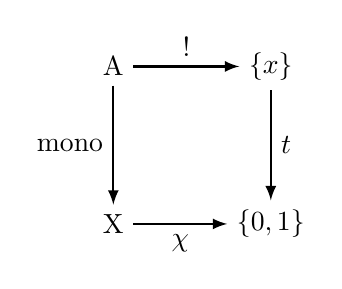
\begin{tikzpicture}[
					      observed/.style = {rectangle, thick, text centered, draw, text width = 6em},
					      latent/.style = {ellipse, thick, draw, text centered, text width = 6em},
					      error/.style ={circle, thick, draw, text centered},
					      confounding/.style = {rectangle, thick, text centered, draw, text width = 6em, minimum width = 5.5in},
					      outcome/.style = {rectangle, thick, draw, text centered, minimum height = 3.5in, text width = 6em},
				      ]
				      \node(TL) at (-1,1){A};
				      \node(BL) at (-1,-1){X};
				      \node(TR) at (1,1){\(\{x\}\)};
				      \node(BR) at (1,-1){\(\{0, 1\}\)};

				      \draw[Arrow](TL)--node[midway, above] {!}(TR);
				      \draw[Arrow](BL)--node[midway, below] {\(\chi \)}(BR);
				      \draw[Arrow](TL)--node[midway, left] {mono}(BL);
				      \draw[Arrow](TR)--node[midway, right] {\(t\)}(BR);
			      \end{tikzpicture}
		      \end{center}
		      meaning the subobject classifier in Sets is the two-element sets and has as morphisms the characteristic function of A. This is indeed a way of classifying all possible subobjects (subsets in the current example) of a given object, it gives the largest subobject of X in which the characteristic function is always true, which in this case is A, via a pullback of \(\Omega \). Hence, generalizing the subobject classifier in Sets gives a way of generalizing the notion of truth-or-false, usually present in the form of whether a set is a subset of another (object and subobject relationship), to more general contexts.
		\item[2)] In the category of topological spaces, if we look for the truth-value object, or subobject classifier, we must start by noticing that the terminal object in this category is a singleton with a topology, known as a \textit{point space}, defined by \((\{x\}, \tau_{x})\) where \(\tau_{x} = \{\emptyset , \{x\}\}\) is the discrete topology for the singleton. Then, taking inspiration from Sets, the classifier maybe could be found by imbuing \(\mathfrak{2} = \{0, 1\}\) with a topology, specifically the trivial topology of all subsets of \(\mathfrak{2}\). Hence, if we are working with a topological space \((X, \tau_{X})\), given a part \((Y, \tau_{Y})\) of it (which would be a subspace of X), the classifier is a continuous function \(\mathrm{true}:(\{x\},\tau_{x})\rightarrow (\mathfrak{2}, \tau_{\mathfrak{2}})\) which checks if ``is this point space of \((X, \tau_{X} )\) also a point space of \((Y, \tau_{Y})\)?''.

		      That continuous function would be the characteristic function, but its continuity fail at the boundary of the topological spaces. As a matter of fact, Top is a category without a subobject classifier exactly because there are non-homeomorphic continuous bijections in it. Later on, we'll see that this makes it so Top is not a Topos! We'll also look into sheaves, which is a type of functor category with something similar to the idea of covers, and the category of sheaves of topological spaces actually does have a subobject classifier.
		\item[3)] For the category of I-indexed families of Sets (an index set I and, for each of its elements k, a set \(S_{k}\)), denoted by \(Sets^{I}\), the subobject classifier is a collection of many of the subobject classifier in Sets repeated, \textit{i.e.}, \((\{0, 1\}_{i})_{i\in I}.\)
	\end{itemize}
\end{example}

There is a way to use the Yoneda Lemma to find a representable way of defining the subobject classifier. For a given object X in a category \(\mathcal{E}\) with finite limits and pullbacks, denote the class of subobjects of X by \(\mathrm{Sub}(X)\). We must also assume that each Sub(X) is a set, so that using a pullback \(f^{*}\) on any map \(X\overbracket[0pt]{\rightarrow}^{f}Y\) also induces a map of sets \(\mathrm{Sub}(Y)\overbracket[0pt]{\rightarrow}^{f^{*}}\mathrm{Sub}(X)\):
\begin{center}
	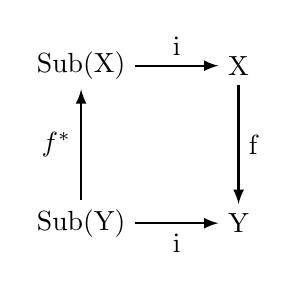
\begin{tikzpicture}[
			observed/.style = {rectangle, thick, text centered, draw, text width = 6em},
			latent/.style = {ellipse, thick, draw, text centered, text width = 6em},
			error/.style ={circle, thick, draw, text centered},
			confounding/.style = {rectangle, thick, text centered, draw, text width = 6em, minimum width = 5.5in},
			outcome/.style = {rectangle, thick, draw, text centered, minimum height = 3.5in, text width = 6em},
		]
		\node(TL) at (-1,1){Sub(X)};
		\node(BL) at (-1,-1){Sub(Y)};
		\node(TR) at (1,1){X};
		\node(BR) at (1,-1){Y};

		\draw[Arrow](TL)--node[midway, above] {i}(TR);
		\draw[Arrow](BL)--node[midway, below] {i}(BR);
		\draw[Arrow](BL)--node[midway, left] {\(f^{*}\)}(TL);
		\draw[Arrow](TR)--node[midway, right] {f}(BR);

	\end{tikzpicture}
\end{center}

In turn, this defines a contravariant functor \(\mathrm{Sub}:\mathcal{E}\rightarrow \mathrm{Sets}\), and a subobject classifier becomes a representation of this functor, meaning there is an object \(\Omega \) in the category \(\mathcal{E}\) with a natural isomorphism between the arrows from objects X in \(\mathcal{E}\) to \(\Omega \), and Sub applied to F:
\[
	\mathrm{Sub}(X)\cong \mathcal{E}(X, \Omega )
\]
If we let \(\mathcal{E}\) be Sets and \(\Omega\) be the 2-element set \(\{0,1\}\), this natural isomorphism becomes
\[
	\mathrm{Sub}(X)\cong \mathrm{Sets}(X, \{0, 1\}),
\]
and, since in Sets the subobjects are subsets, we have a natural isomorphism between the subsets of X and the maps from X to \(\{0, 1\}\) - subsets of X correspond naturally to maps \(X\rightarrow \{0,1\}.\)

Further exploring this correspondence, let's check if it coincides with the subobject classifier in any category with finite limits \(\mathcal{E}\). Given the functor \(\mathrm{Sub}:\mathcal{E}^{\mathrm{op}}\rightarrow \mathrm{Sets}\) (which is the same as what was defined above), every representation of Sub according to the Yoneda Lemma is given exactly from an universal morphisms as in
\[
	\mathcal{E}(-, \Omega )\cong \mathrm{Sub}(-),
\]
where \(\Omega \) must satisfy the universal morphism property \(\langle \Omega , t:T \rightarrowtail \mathrm{Sub}(\Omega ) \rangle\), where T is the terminal object, which means any arrow from \(T\) to \(\mathrm{Sub}(\Omega )\) factors uniquely through t. Thus, for an object X in \(\mathcal{E}\), we have the following correspondence: \(\mathcal{E}^{\mathrm{op}}(\Omega , X)\cong \mathrm{Sub}(X)\), or
\begin{center}
	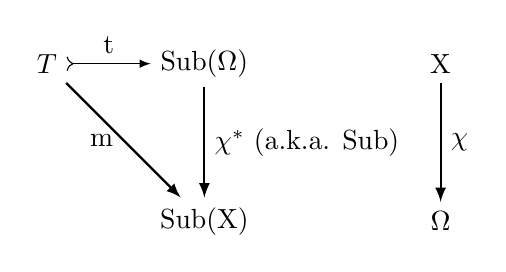
\begin{tikzpicture}[
			observed/.style = {rectangle, thick, text centered, draw, text width = 6em},
			latent/.style = {ellipse, thick, draw, text centered, text width = 6em},
			error/.style ={circle, thick, draw, text centered},
			confounding/.style = {rectangle, thick, text centered, draw, text width = 6em, minimum width = 5.5in},
			outcome/.style = {rectangle, thick, draw, text centered, minimum height = 3.5in, text width = 6em},
		]
		\node(TL) at (-1,1){\(T\)};
		\node(BR) at (1,-1){Sub(X)};
		\node(TR) at (1,1){Sub(\(\Omega \))};

		\node(TTR) at (4,1){X};
		\node(BBR) at (4,-1){\(\Omega \)};

		\draw[>-latex](TL)--node[midway, above] {t}(TR);
		\draw[Arrow](TL)--node[midway, left] {m}(BR);
		\draw[Arrow](TR)--node[midway, right] {\(\chi ^{*}\) (a.k.a. Sub)}(BR);
		\draw[Arrow](TTR)--node[midway, right] {\(\chi\)}(BBR);

	\end{tikzpicture}
\end{center}
this means that for every objects X of \(\mathcal{E}\) and element m in Sub(X), there is a unique map \(\chi :X\rightarrow \Omega \) such that
\[
	\chi^{*}\circ t = m,
\]
and using the result that arrows out of a terminal object T are monomorphisms together with the usage of a pullback, another result can be used to show that this is equivalent to saying that \(\Omega \) is a subobject classifier.

\section{Sheaves and Presheaves}

To understand what is a sheaf, one must understand what is a presheaf. Sequentially, to understand what is a presheaf, we can start from the topological meaning of the term.
\begin{def*}
	Let X be a topological space. For every open set \(U\subseteq X\), a \textbf{presheaf} \(\mathcal{E}\) gives a set \(\mathcal{E}(U)\) such that for every inclusion of open sets \(V\subseteq U\subseteq X\), we have a map \(\rho_{V}^{U}:\mathcal{E}(U)\rightarrow \mathcal{E}(V)\) known as the \textbf{restriction} such that
	\begin{itemize}
		\item[a)] For any open set \(U\subseteq X\), \(\rho_{U}^{U}=\mathrm{Id} \);
		\item[b)] For all open sets \(W\subseteq U\subseteq V\), \(\rho_{W}^{U}=\rho_{W}^{V}\circ \rho_{V}^{U}\).
	\end{itemize}
\end{def*}
The definition might seem daunting at first, but we can look at it through a category theorists' eyes. First of all, we begin with objects in Top - V and U are open sets of X - such that there is a morphism ``inclusion'' between them, i.e., \(V\subseteq U (V\overbracket[0pt]{\rightarrow}^{\subseteq }U)\).
Then, we begin to look at objects in the category of Sets: V and U become elements in the image of E, which takes open sets, turns them into sets, and gives another morphism between them; however, the direction is reversed, since \(\rho_{V}^{U}:\mathcal{E}(U)\rightarrow \mathcal{E}(V)\). In other words, up until this point, the presheaf is a functor from reversed Top into Sets \(\mathcal{E}:\mathrm{Top}^{\mathrm{op}}\rightarrow \mathrm{Sets}\).

There are two other properties, and we can in fact translate them to the categorical language: For the first item, it only means that the functor preserves the identity, which is in fact one of the properties of a functor, and the second one is a composition law. Hence, we can state categorically that
\begin{def*}
	A \textbf{presheaf} on a small category \(\mathcal{C}\) is a covariant functor
	\[
		F:\mathcal{C}^{\mathrm{op}}\rightarrow \mathrm{Sets}.\quad \square
	\]
\end{def*}
Equivalently, it can be thought of as a contravariant functor from a small category \(\mathcal{C}\) to Sets.

Furthermore, and quite conveniently, we can also think of a category of presheaves, one in which objects are presheaves, and the morphisms between them are natural transformations between functors - they satisfy composition laws and have an identity. From the examples seen during the classes, this makes up a specific example of the \textit{Functor Category}, and thus, following the notation of \(\mathcal{A}^{\mathcal{C}}\) for the category of functors from category \(\mathcal{A}\) to category \(\mathcal{C}\), we may denote the category of presheaves by \(\mathrm{Sets}^{\mathcal{C}^{\mathrm{op}}}\). Its objects are the functors \(F:\mathcal{C}^{\mathrm{op}}\rightarrow \mathrm{Sets}\), and the morphisms are natural transformations between them. A very nice fact about this category is that it is cartesian closed whenever \(\mathcal{C}\) is small, which, as we'll see later, makes working with different Topoi much more feasible.

\begin{example}
	\begin{itemize}
		\item[1)] Consider the small category \(\mathrm{Top}\) of topological spaces. The presheaves on it are given generally by
		      \[
			      Psh:\mathrm{Top}^{\mathrm{op}}\rightarrow \mathrm{Sets},
		      \]
		      which means that for each continuous function between topological spaces \(f:(X, \tau_{X})\rightarrow (Y, \tau_{Y})\), applying F yields a function from Y to X \(F(f):Y\rightarrow X\). The category of presheaves on topological spaces \(\mathrm{Sets}^{\mathrm{Top}^{\mathrm{op}}}\) is cartesian closed, while Top is not!
	\end{itemize}
\end{example}

Knowing at least intuitively what is a presheaf, the next step as mentioned before is to look at \textit{Sheaves.} We can follow a similar reasoning, starting from a subject in which there is a definion of a Sheaf, then try to generalize it for categories. As a matter of fact, once again it is useful to turn to topology:

\begin{def*}
	A \textbf{sheaf} is a presheaf with the additional property that for every open set U and every open cover \(\{U_{i}\}\) of U (\(U\subseteq \bigcup_{i\in I}^{}U_{i},\; U_{i}\) are open), IF there exist functions \(f_{i}\in \mathcal{E}(U)\) in the presheaf of U such that
	\[
		\rho_{U_{i}\cap U_{j}}^{U_{i}}(f_{i})=\rho_{U_{i}\cap U_{j}}^{U_{j}}(f_{j})
	\]
	for all pairs (i, j), then there is a unique f in the presheaf of U such that \(\rho_{U_{i}}^{U}(f) = f_{i}\) for all i. \(\square\)
\end{def*}
This property of sheaves essentially means that as long as you can cover the open set, then any functions in the presheaf that coincide after being restricted to the intersection of that cover have their action described uniquely by a single function with different types of domain restrictions in the cover.

Hence, the values of the functions on the presheaf of each covering component can be recovered by looking at a unique, single function on the presheaf of the set being covered. It mainly boils down to how we can translate the restriction and its condition, as well as the idea of covers, to categorical language. Hence, once a few definitions have been laid down, we shall go and give the more general definition.
\begin{def*}
	Let \(\mathcal{C}\) be a category and A be an object of \(\mathcal{C}\). A \textbf{cover on A} is a collection of morphisms
	\[
		\{U_{i}\overbracket[0pt]{\rightarrow}^{}U\}_{i\in I}.
	\]
	the collection of morphisms is called a \textbf{covering family}. \(\square\)
\end{def*}
\begin{def*}
	Using the notation above, a \textbf{coverage} on \(\mathcal{C}\) is a function assigning to each object U of \(\mathcal{C}\) a covering family with the following additional property: if \(\{f_{i}:U_{i}\rightarrow U\}_{i\in I}\) is a covering family and \(g:U\rightarrow V\) is a morphism, then there exists a covering family \(\{h_{j}:V_{j}\rightarrow V\}\) such that each composite \(gh_{j}\) factors through some \(f_{i}\):
	\begin{center}
		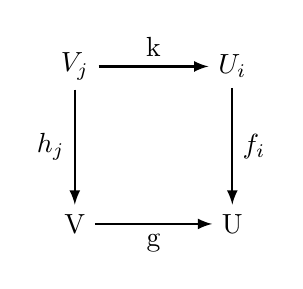
\begin{tikzpicture}[
				observed/.style = {rectangle, thick, text centered, draw, text width = 6em},
				latent/.style = {ellipse, thick, draw, text centered, text width = 6em},
				error/.style ={circle, thick, draw, text centered},
				confounding/.style = {rectangle, thick, text centered, draw, text width = 6em, minimum width = 5.5in},
				outcome/.style = {rectangle, thick, draw, text centered, minimum height = 3.5in, text width = 6em},
			]
			\node(TL) at (-1,1){\(V_{j}\)};
			\node(BL) at (-1,-1){V};
			\node(TR) at (1,1){\(U_{i}\)};
			\node(BR) at (1,-1){U};

			\draw[Arrow](TL)--node[midway, above] {k}(TR);
			\draw[Arrow](BL)--node[midway, below] {g}(BR);
			\draw[Arrow](TL)--node[midway, left] {\(h_{j}\)}(BL);
			\draw[Arrow](TR)--node[midway, right] {\(f_{i}\)}(BR);

		\end{tikzpicture}
	\end{center}
	which means that for all \(f_{i}\) and g, there exists an \(h_{i}\) such that there exists i and k for which
	\[
		g\circ h_{j} = k\circ f_{i}. \quad \square
	\]
\end{def*}

\begin{def*}
	A \textbf{site} is a category equipped with a coverage. \(\square\)
\end{def*}

Open covers are then just the families for covering families, which are categorical covers in which the morphism is the usual inclusion of sets, for instance, and a coverage would be the composition rule that allows morphisms of covering families to also be covering families.

We still have to generalize the other property of a topological sheaf, namely the restriction and its condition, as previously called; with respect to this one, we start with the definition of a \textit{sieve}. In the world of people and objects (also known as the real world), a sieve works as an object which lets liquids or small particles through, but holds off bigger particles (think of the thing one does when straining water from pasta).

In a sense, the categorical idea of a sieve is not that far off, but instead of sifting out water from pasta, or big boulders of flour from small ones, you sift out from representable functors, \textit{i.e.} functors such that there exists a natural isomorphism \(\theta :\mathrm{Hom}_{\mathcal{C}}(-, C)\rightarrow F\), where \(\mathcal{C}\) is an arbitrary category and C one of its elements, subobjects which form a cover of a coverage, essentially separating unwanted subobjects (the water) from the desired ones (the pasta). Since this is a very weird analogy, let's now take a look at the mathematical definition of a sieve:

\begin{def*}
	A functor \(F:\mathcal{C}\rightarrow \mathcal{B}\) is a \textbf{discrete fibration} if for every object C in \(\mathcal{C}\), and every morphism \(g:B\rightarrow F(C)\) in \(\mathcal{B}\), there is a unique morphism \(h:D\rightarrow C\) in \(\mathcal{C}\) such that
	\[
		F(h) = g.\quad \square
	\]
\end{def*}

\begin{def*}
	A \textbf{sieve S} in a small category \(\mathcal{C}\) is a functor \(S\hookrightarrow \mathcal{C}\) that is both fully faithful and a discrete fibration. \(\square\)
\end{def*}

\begin{def*}
	Let \((\mathcal{C}, J)\) be a site, where \(\mathcal{C}\) is a small category equipped with a coverage J. A presheaf \(A\in \hat{\mathcal{C}}\) is called a \textbf{sheaf} if for every covering family \(\{p_{i}:U_{i}\rightarrow U\}_{i\in I}\) in J, and for every tuple \((s\in A(U_{i}))_{i\in I}\) in the presheaf of \(U_{i}\), they satisfy the property that
	\begin{itemize}
		\item for all j, k in I and all morphisms \(f:K\rightarrow U_{j}\), \(g:K\rightarrow U_{k}\) in \(\mathcal{C}\) with \(p_{j}\circ f=p_{k}\circ g\) we have \(A(f)(s_{j})=A(g)(s_{k})\) belongs to A(K),
	\end{itemize}
	there is a unique element s in the presheaf of U such that
	\[
		A(p_{i})(s)=s_{i}
	\]
	for all i in I.

	Another way to put it is to ask that for every cover \(\{p_{i }:U_{i}\rightarrow U\}\), the diagram
	\[
		\mathcal{A}(U)\rightarrow \prod\limits_{i}^{}A(U_{i})\rightrightarrows \prod\limits_{j, k}^{} \mathrm{PSh}_{\mathcal{C}}(j(U_{j}))\times_{j(U)}j((U_{k}), A)
	\]
	is an equalizer, where \(\mathrm{Psh}(-, A)\) is the hom-functor (\(\mathrm{Hom}_{\mathcal{C}}:\mathcal{C}\times \mathcal{C}^{\mathrm{op}}\rightarrow \mathrm{Sets}\)) \(\square\)
\end{def*}

At a glance, that seems like a lot to unpack, but it's just a matter of time and will. The covering family part and the tuple in the presheaf means essentially that we're taking a bunch of objects in the presheaf of an element in the covering family.

As for the property right next to it, that is translating the ``gluing'' part from its topological counterpart: we can glue morphisms that coincide in the members of the covering family together, even if they are not the same members, once they are in the sheaf, as long as they leave from the same object.

To wrap it up, we ask for a \textit{unique} way of gluing these morphisms together, such that if you know what that unique glue is in the presheaf of the whole object, you can recover its form as it is inside whichever object in its covering family you want. In other words, we are looking for presheaves that are characterized by local properties.

It is worth mentioning that sheaves also form a functor category, Sh, whose objects are sheaves and the morphisms are natural transformations between them. It is a subcategory of the category of presheaves \(\mathcal{A}^{\mathcal{C}}\), and hence it makes sense to denote it by \( \mathrm{Sh}(\mathcal{C})\).

\begin{example}
	\begin{itemize}
		\item[1)] Given a topological sapce X, let \(\mathcal{O}(X)\) be the poset of open subsets of X. Then, the following functor is a sheaf with action being intersection:
		      \[
			      \mathcal{O}:\mathcal{O}(X)^{\mathrm{op}}\rightarrow \mathrm{Sets},\quad \mathcal{O}(U) = \{W\in \mathcal{O}(X): W\subseteq U\},
		      \]
		\item[2)] Fix a continuous map \(f:Y\rightarrow X\) and, for each open set U of X, let
		      \[
			      S_{f}(U)=\{\sigma:U\rightarrow Y: f(\sigma(x))=x \forall x\in U\}.
		      \]
		      Under restriction, this is a sheaf.
		\item[3)] For each open set \(U\in \mathcal{O}(X)\), the representable presheaf \(\mathcal{O}(-, U):\mathcal{O}(X)^{\mathrm{op}}\rightarrow \mathrm{Sets}\) is a sheaf.
		\item[4)] For a presheaf that is not a sheaf, one may think of bounded functions in the complex plane, which break apart in the uniqueness property thanks to Liouville's theorem.
	\end{itemize}
\end{example}

\section{Elementary Topos and Sets as a Topos}

Taking into account wish for expanding the ideas behind Sets, we'll use them as main motivation and example while studying topoi. Roughly speaking,

\begin{def*}
	A \textbf{Topos} or an \textbf{Elementary Topos} is a cartesian closed category with finite limits and a subobject classifier. \(\square\)
\end{def*}

More than just defining what are topoi, we'll explore a few examples and then move on to looking at Sets as a topos, since it will give us clues about the development of a topos theory. Usually, the hardest part in determining whether or not a category is a topos ends up being its subobject classifier.

\begin{example}
	\begin{itemize}
		\item[1)] For any set I, the category \(\mathrm{Sets}^{I}\) of I-indexed families of sets is a topos whose subobject classifier is the constant family \((2)_{i\in I}\), where 2 is a two-element set. Essentially a family of I-indexed characteristic functions;
		\item[2)] For any group G, the category \(\mathrm{Sets}^{G}\) of left G-sets, \textit{i.e.} a set X equipped with a group action \(g:G\times X\rightarrow X \), is a topos. The subobject classifier is the set with two-elements together with the trivial G-action \(e_{G}:G\times X\rightarrow X\) so that \(e_{G}x = x\) for all x in X.
		\item[3)] If \(\mathbb{A}\) is any \textit{small category} (its collection of objects is a set), then the category of presheaves \(\hat{\mathbb{A}}=\mathrm{Sets}^{\mathbb{A}^{\mathrm{op}}}\) on \(\mathbb{A}\) is a topos. We can use a process similar to how we used the Yoneda Lemma for an equivalent definition of the subobject classifier to find out how they look in this example. Given an object A in \(\mathbb{A},\) we have
		      \[
			      \hat{\mathbb{A}}(\mathbb{A}(-, A), \Omega )\cong \mathrm{Sub}(\mathbb{A}(-, A)),
		      \]
		      which is representable via \(\Omega \), so that
		      \[
			      \Omega(A)\cong \hat{\mathbb{A}}(\mathbb{A}(-, A), \Omega )\cong \mathrm{Sub}(\mathbb{A}(-, A)),
		      \]
		      Here, the subobjects of \(\mathbb{A}(-, A)\) are subfunctors, which means the subobject classifier for a presheaf must be the set of subfunctors of \(\mathbb{A}(-, A)\). This is the definition of a \textbf{sieve} on A, a collection of maps into A satisfying a certain condition.
	\end{itemize}
\end{example}

This idea of topos as generalized sets is not just for the sake of appreciation, but it actually works as a useful tool in category theory. We can also speak of other generalized structures that appear inside Sets, and the first step towards that direction is to understand what makes Sets a special Topos:
\begin{itemize}
	\item[1)] its terminal object is a separator: given morphisms f, g from X to Y in Sets, if \(f\circ x = g\circ x\) for all \(x:1\rightarrow X\), then f = g;
	\item[2)] Sets is not equivalent to the terminal category (the one with a single object and a single morphism pointing to that object);
	\item[3)] Set has a \textit{natural numbers object} (which is, in fact, the usual natural numbers. See below for the definition of a natural numbers object);
	\item[4)] For any epimorphism \(e:X\rightarrowtail  Y\), there exists a map \(m:Y\rightarrow X\) such that \(e\circ m = 1_{Y}\).
\end{itemize}
Property number four is exactly the Axiom of Choice, since it entails that for each object Y, one can pick an element y in it such that it is an element of \(e^{-1}\{y\}\), and for that reason any category in which epimorphisms split is said to satisfy the axiom of choice.

\begin{def*}
	Let \(\mathcal{E}\) be a category with a temrinal object 1. A \textbf{natural number object in }\(\mathcal{E}\) is a triplet (N, 0, s) with N being an object of \(\mathcal{E}\), \(0:1\rightarrow N\), and \(s:N\rightarrow N\) such that the following diagram commutes:
	\begin{center}
		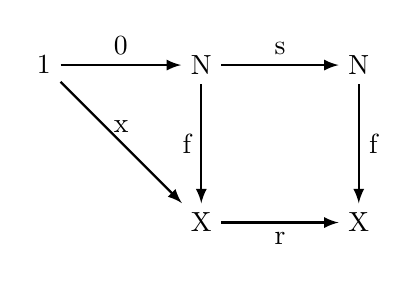
\begin{tikzpicture}[
				observed/.style = {rectangle, thick, text centered, draw, text width = 6em},
				latent/.style = {ellipse, thick, draw, text centered, text width = 6em},
				error/.style ={circle, thick, draw, text centered},
				confounding/.style = {rectangle, thick, text centered, draw, text width = 6em, minimum width = 5.5in},
				outcome/.style = {rectangle, thick, draw, text centered, minimum height = 3.5in, text width = 6em},
			]
			\node(TL) at (-1,1){N};
			\node(TTL) at (-3,1){1};
			\node(BL) at (-1,-1){X};
			\node(TR) at (1,1){N};
			\node(BR) at (1,-1){X};

			\draw[Arrow](TTL)--node[midway, above] {0}(TL);
			\draw[Arrow](TTL)--node[midway, above] {x}(BL);
			\draw[Arrow](TL)--node[midway, above] {s}(TR);
			\draw[Arrow](BL)--node[midway, below] {r}(BR);
			\draw[Arrow](TL)--node[midway, left] {f}(BL);
			\draw[Arrow](TR)--node[midway, right] {f}(BR);

		\end{tikzpicture}
	\end{center}
\end{def*}

and that was was Lawvere suggested to take as a definition of \textit{a} category of Sets - any well-pointed topos satisfying Choice and which has a natural numbers object. No need for ZFC.

To better understand the power that comes from having an axiomatization from maps between objects, we can look at a category's internal language, which is, \textit{very} roughly speaking, a way to talk about stuff happening inside a category using spoken language. It helps reformulate definitions without diagrams, prove stuff, and so on. Let's have a look at it.

\begin{def*}
	Let \(\mathcal{C}\) be a category and X be one of its objects. A \textbf{generalized element} of X is a map in \(\mathcal{C}\) whose codomain is X. We say that a generalized element \(x:S\rightarrow X\) is of \textbf{Shape S}; equivalently, we call it an \textbf{S-shaped element of X}. \(\square\)
\end{def*}
In the case where S is a terminal object, we call the generalized element \(x:S\rightarrow X\) a \textbf{global element.}

There is a very nice thing that is given rise thanks to the notion of a generalized element, which is sort of a generalization of functions. To see that, consider a morphism \(f:X\rightarrow Y\) in \(\mathcal{C}\); a generalized element x of X gives rise to a generalized element of Y via the composition
\[
	S\overbracket[0pt]{\rightarrow}^{x}X\overbracket[0pt]{\rightarrow}^{f}Y,
\]
and that generalized element is \(f\circ x\), but it can be thought of as f(x). This also allows us to check when two morphisms are the same: given two morphisms \(f:X\rightarrow Y\) and \(g:X\rightarrow Y\), suppose f = g. Then,

\[
	f\circ x = g \circ x
\]

for all generalized elements of X. On the other hand, if \(f\circ x = g\circ x\) for all generalized elements x of X, then in particular it is true for \(x = 1_{X}\), so that
\[
	f\circ 1_{X} = g\circ 1_{X} \Rightarrow f = g.
\]
What this means is that two morphisms f and g only coincide if they are the same for all generalized elements of their domain.

This kind of reasoning is not just for the sake of generality, it is also \textit{very} useful in proving statements or defining stuff inside categories as a techique that goes along diagram hunting, which is why it is known as a category's \textbf{internal language}. For example, in a category with finite products, we can take generalized elements of exponentials \(X^{Y}\) and form a subobject as
\[
	\{x\in X: fx = gx\},
\]
which will be exactly the non-diagram version of the equalizer of \(X\overbracket[0pt]{\rightarrow}^{f}Y\) and \(X\overbracket[0pt]{\rightarrow}^{g}Y\). For reference, when defining diagramatically,

\begin{def*}
	The \textbf{equalizer} consists of an object E and a morphism \(\varepsilon :E\rightarrow X\) satisfying \(f\circ \varepsilon = g\circ \varepsilon \), and such that given any object O and morphism \(m:O\rightarrow X\) if \(f\circ m=g\circ m\), then there exists a unique morphism \(u:O\rightarrow E\) such that \(\varepsilon \circ u=m\). In other words, the following diagram commutes:
	\begin{center}
		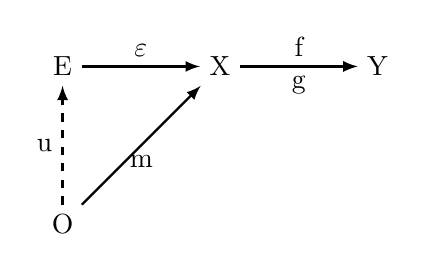
\begin{tikzpicture}[
				observed/.style = {rectangle, thick, text centered, draw, text width = 6em},
				latent/.style = {ellipse, thick, draw, text centered, text width = 6em},
				error/.style ={circle, thick, draw, text centered},
				confounding/.style = {rectangle, thick, text centered, draw, text width = 6em, minimum width = 5.5in},
				outcome/.style = {rectangle, thick, draw, text centered, minimum height = 3.5in, text width = 6em},
			]
			\node(TL) at (-1,1){E};
			\node(BL) at (-1,-1){O};
			\node(TR) at (1,1){X};
			\node(BR) at (3,1){Y};

			\draw[Arrow](TL)--node[midway, above] {\(\varepsilon \)}(TR);
			\draw[Arrow](BL)--node[midway, below] {m}(TR);
			\draw[Arrow, dashed](BL)--node[midway, left] {u}(TL);
			\draw[Arrow](TR)--node[midway, above] {f}(BR);
			\draw[Arrow](TR)--node[midway, below] {g}(BR);

		\end{tikzpicture}
	\end{center} \(\square\)
\end{def*}
with respect to the help in proving things, consider, for instance, internal groups in a finite product category \(\mathcal{E}\):

\begin{def*}
	A group in \(\mathcal{E}\) is an object X together with maps
	\[
		m:X\times X\rightarrow X,\: i:X\rightarrow X,\: e:1\rightarrow X
	\]
	satisfying the usual axioms of group theory. \(\square\)
\end{def*}
Usually, said axioms are stated in terms of diagrams, and as such can be quite confusing:
\begin{center}[Associativity]
	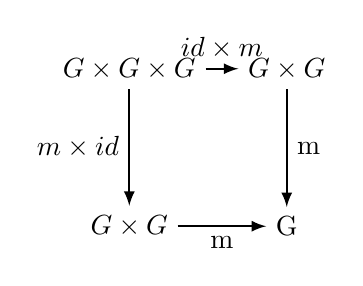
\begin{tikzpicture}[
			observed/.style = {rectangle, thick, text centered, draw, text width = 6em},
			latent/.style = {ellipse, thick, draw, text centered, text width = 6em},
			error/.style ={circle, thick, draw, text centered},
			confounding/.style = {rectangle, thick, text centered, draw, text width = 6em, minimum width = 5.5in},
			outcome/.style = {rectangle, thick, draw, text centered, minimum height = 3.5in, text width = 6em},
		]
		\node(TL) at (-1,1){\(G\times G\times G\)};
		\node(BL) at (-1,-1){\(G\times G\)};
		\node(TR) at (1,1){\(G\times G\)};
		\node(BR) at (1,-1){G};

		\draw[Arrow](TL)--node[midway, above] {\(id\times m\)}(TR);
		\draw[Arrow](BL)--node[midway, below] {m}(BR);
		\draw[Arrow](TL)--node[midway, left] {\(m\times id\)}(BL);
		\draw[Arrow](TR)--node[midway, right] {m}(BR);

	\end{tikzpicture}
\end{center}

\begin{center}[Unitality]
	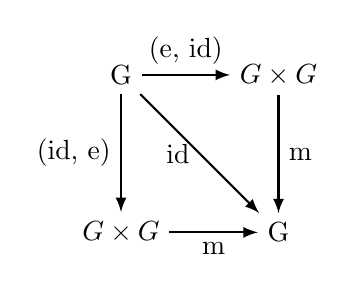
\begin{tikzpicture}[
			observed/.style = {rectangle, thick, text centered, draw, text width = 6em},
			latent/.style = {ellipse, thick, draw, text centered, text width = 6em},
			error/.style ={circle, thick, draw, text centered},
			confounding/.style = {rectangle, thick, text centered, draw, text width = 6em, minimum width = 5.5in},
			outcome/.style = {rectangle, thick, draw, text centered, minimum height = 3.5in, text width = 6em},
		]
		\node(TL) at (-1,1){G};
		\node(BL) at (-1,-1){\(G\times G\)};
		\node(TR) at (1,1){\(G\times G\)};
		\node(BR) at (1,-1){G};

		\draw[Arrow](TL)--node[midway, above] {(e, id)}(TR);
		\draw[Arrow](BL)--node[midway, below] {m}(BR);
		\draw[Arrow](TL)--node[midway, left] {(id, e)}(BL);
		\draw[Arrow](TL)--node[midway, left] {id}(BR);
		\draw[Arrow](TR)--node[midway, right] {m}(BR);
	\end{tikzpicture}
\end{center}

In terms of a generalized element g of G, this means
\[
	m((id(g), e())) = g
\]

\begin{center}[Invertibility]
	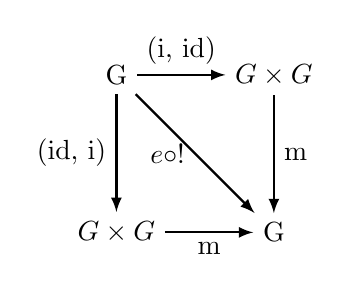
\begin{tikzpicture}[
			observed/.style = {rectangle, thick, text centered, draw, text width = 6em},
			latent/.style = {ellipse, thick, draw, text centered, text width = 6em},
			error/.style ={circle, thick, draw, text centered},
			confounding/.style = {rectangle, thick, text centered, draw, text width = 6em, minimum width = 5.5in},
			outcome/.style = {rectangle, thick, draw, text centered, minimum height = 3.5in, text width = 6em},
		]
		\node(TL) at (-1,1){G};
		\node(BL) at (-1,-1){\(G\times G\)};
		\node(TR) at (1,1){\(G\times G\)};
		\node(BR) at (1,-1){G};

		\draw[Arrow](TL)--node[midway, above] {(i, id)}(TR);
		\draw[Arrow](BL)--node[midway, below] {m}(BR);
		\draw[Arrow](TL)--node[midway, left] {(id, i)}(BL);
		\draw[Arrow](TL)--node[midway, left] {\(e\circ !\)}(BR);
		\draw[Arrow](TR)--node[midway, right] {m}(BR);

	\end{tikzpicture}
\end{center}

As far as generalized elements g in G go, this would be
\[
	m(id(g), i(g)) = e.
\]

But using the internal language, it is just a matter of rewriting the usual group axioms for all generalized elements x, y, z of X of the same shape. Another example would be the definition of, say, a terminal object:
\begin{def*}
	Given a category \(\mathcal{C}\), an object 1 is said to be terminal if every object X of \(\mathcal{C}\) has a unique morphism \(!:X\rightarrow 1\). \(\square\)
\end{def*}
rewritten in terms of generalized elements, this means that an object 1 is terminal if there is exactly one X-shaped element x in 1 for all objects X: it is the general version of a one-point set!

In particular, because topoi can be viewed as generalized Sets, any proof that is constructive by nature in Sets can just be copied down step-by-step in an arbitrary topos. This is thus a way to get a different axiomatization of Set-theory other than ZFC, known as the Elementary Theory of the Category of Sets, which was presented earlier.

\section{Maps Between Topoi}

Having in mind the algebraic geometry origins of topos theory, a very nice way of finding out properties about topoi to test out is by generalizing ideas from geometry or topology to topoi.

As per usual, nice maps between two toposes must preserve the nice properties they have. These maps are called \textit{logical morpphisms}. To illustrate this techique for property disccvering and to start with the discussion of maps between topoi, we'll derive a notion of map of toposes that are more useful\footnote{And easier for me to understand, since I tried understanding logical morphisms but I got nowhere after seeing something known as Heyting algebras (?). They will be mentioned later though.} than logical morphisms,

Every map in the category of topological spaces \(f:X\rightarrow Y\) induces an adjunction (which, recall, is a pair of dual morphisms) via
\[
	Sh(X)\overbracket[0pt]{\rightarrow}^{f_{*}}Sh(Y) \quad\&\quad Sh(Y)\overbracket[0pt]{\rightarrow}^{f^{*}}Sh(X).
\]
The right adjoint \(f_{*}:Sh(X)\rightarrow Sh(Y)\) is constructed by pulling back a sheaf of an open space V of Y:
\[
	(f_{*}F)(V) = F(f^{-1}V),
\]
and the left one \(f^*\) is harder to define, but there Re some results that can be used for it and that fall out of the goal we have here. A fact that ends up as result is that \(f ^{*}\) preserves finite limits. Hence, we can use this to define how a morphism that is like a continuous map would look like in terms of topos theory:

\begin{def*}
	Let \(\mathcal{E}\) and \(\mathcal{F}\) be two topoi. A \textbf{geometric morphism} \(f:\mathcal{E}\rightarrow \mathcal{F}\) is an adjunction of the form
	\[
		\mathcal{E}\overbracket[0pt]{\rightarrow}^{f_{*}}\mathcal{F} \quad\&\quad \mathcal{F}\overbracket[0pt]{\rightarrow}^{f^{*}}\mathcal{E},
	\]
	in which the left adjoint \(f ^{*}\) preserves finite limits. The right adjoint \(f_{*}\) is called the \textbf{direct image} part of f, and \(f^{*}\) is the \textbf{inverse image part}. \(\square\)
\end{def*}

With that, we have a category of toposes, Topoi, whose objects are, well, topoi, and the morphisms are geometric morphisms. Moreover, the construction above we used to find the definition for the geometric morphism also gives a functor that is full and faithful between Topoi and Top.

What would that functor be? We are taking \textit{topological spaces} with \textit{continuous functions} between them, and getting \textit{topoi} with \textit{geometric morphisms} between them. The objects inside topoi are still categories by definition of topoi, so we are in fact taking topological spaces and turning them into categories with something more. By the process made above, we started out with topological space X and Y, studied their sheaves Sh(X) and Sh(Y), and generalized to topoi; hence, the functor is exactly
\[
	\mathrm{Sh}:\mathrm{Top}\rightarrow \mathrm{Topoi},
\]
so it allows one to study topoi as sheaves of topological spaces in some cases, which gives a hint at the second way of viewing topoi: generalized spaces.

Another instance where geometric morphisms appear is in something called \textbf{sheafification}: given a topological space X, since Sh(X) is a subcategory of \(\mathrm{Sets}^{X^{\mathrm{op}}}\), the inclusion \(\mathrm{Sh}(X)\overbracket[0pt]{\rightarrow}^{h}\mathrm{Sets}^{X^{\mathrm{op}}}\) has a finite-limite-preserving left adjoint - an inverse part of its geometric morphism.

They also allow for generalization of other geometric constructs, such as points:

\begin{def*}
	A \textbf{point} of a topos \(\mathcal{E} \) is a geometric morphism \(\mathrm{Sets}\rightarrow \mathcal{E}\)
\end{def*}

The reason for such a definition also follows a process of generalizing from some topological notion. In topology, the points of a topological space X can be thought of as morphisms \(p:\{x\}\rightarrow X\). Then, we can apply the functor \(\mathrm{Sh}\) from above to get a point as a morphism
\[
	\mathrm{Sh}(\{x\})\rightarrow \mathrm{Sh}(X).
\]
However, the sheaf of a singleton is equivalent to its presheaf, and the presheaf of a singleton is just Sets; hence the definition.

Regarding logical morphisms, they are functors preserving finite limits, exponentials, and the subobject classifier, and they appear more when studying models of higher-order theories (\textit{i.e.} theories that go beyond quantifying over elements of a set, such as type theory), since you will actually want to preserve everything possible from a topos to another, and they are the mathemaitcal place where higher-order theories are done.

Based on the above, one can think of topoi as coming in three major flavors:
\begin{itemize}
	\item[1)] Generalized sets (from set-theory);
	\item[2)] Generalized spaces (from geometry);
	\item[3)] Generalized logic (from algebra).
\end{itemize}
and as much as I'd love to discuss the latter two in much more detail, I'm bounded by my own ignorance and uncertainty; as such, I can't compromise on rewriting too much about them (I did a little bit about item 2) since that'd be pretty much misinformation or just a copy-and-paste from other places. Not very nice. Still, I hope the discussion about generalized sets was enjoyable, dear reader!

\begin{thebibliography}{99}
	\bibitem{centazzo} CENTAZZO, C. and VITALE, E. M. Available at: \url{https://perso.uclouvain.be/enrico.vitale/chapter7.pdf}. Université Catholique de Louvain, Belgium. Access date: February 7th, 2025.

	\bibitem{lawvere2009}LAWVERE, F. W. and SCHANUEL, S. H. \textbf{Conceptual Mathematics, 2nd Edition:} A first introduction to categories. Cambridge University Press, Cambridge.

	\bibitem{leinster2011}LEINSTER, T. An informal introduction to topos theory. \textbf{Publications of the nLab}, v.1, n.1, 2011. Available at: \url{http://ncatlab.org:80/publications/published/Leinster2011}. Access date: January 11th, 2025.

	\bibitem{pullback}NLAB. \textbf{Pullback}. Available at: \url{https://ncatlab.org/nlab/show/pullback}. Access date: February 1st, 2025.

	\bibitem{groupobject}NLAB. \textbf{Group Object}. Available at: \url{https://ncatlab.org/nlab/show/group+object}. Access date: February 5th, 2025.

	\bibitem{topos}NLAB. \textbf{Topos}. Available at: \url{https://ncatlab.org/nlab/show/topos} Access date: January 15th, 2025.

	\bibitem{stern2013}STERN, J. M. \textbf{Cognitive Constructivism and the Epistemic Significance of Sharp Statistical Hypotheses in Natural Sciences}. São Paulo: Instituto de Matemática e Estatística da Universidade de São Paulo, 2013. Available at: \url{https://www.ime.usp.br/~jmstern/wp-content/uploads/2020/10/evli.pdf}. Access date: February 3rd, 2025.

	\bibitem{schapira2023}SCHAPIRA, P. \textbf{An introduction to Categories and Sheaves}. Paris: Institut de Math´ematiques de Jussieu-Paris Rive Gauche, 2023. Available at: \url{https://webusers.imj-prg.fr/~pierre.schapira/LectNotes/CatShv.pdf}. Access date: February 3rd, 2025.

	\bibitem{speyer2013}TENGEN, Z. \textbf{NOTES FOR JANUARY 13}. Available at: \url{https://dept.math.lsa.umich.edu/~speyer/632Old/jan-13.pdf}. Access date: January 09th, 2025.

\end{thebibliography}

\end{document}
